%!TEX root = ../paper.tex
In this section, experiments are performed to evaluate the performance of three similarity metrics previously discussed in Section~\ref{sec:tkdebackground}: Makiyama's similarity~\cite{makiyama2015text}, Aligon's similarity~\cite{aligon2014similarity} and Aouiche's similarity~\cite{aouiche2006}. 
Each of these similarity metrics is implemented in Java and evaluated using the three clustering validation measures discussed in subsection~\ref{subsec:validation}.
In particular, these three similarity metrics are evaluated on their ability to capture the tasks performed by SQL queries.
In addition, the effectiveness of the feature engineering step introduced in Section~\ref{sec:system} is also introduced which helps to understand how query similarity can be improved by applying this step on the SQL query.
Feature engineering is examined closer by breaking it down to different modules and analyze the effect of each module on capturing the tasks performed by queries.

\subsection{Evaluation on SQL similarity metrics}
\label{subsec:experiments}

In the first experiment, three similarity metrics mentioned in Section~\ref{sec:tkdebackground} are evaluated.
The aim of the experiment is to evaluate which similarity metric can best capture the task performed by each query.

\begin{figure*}[h!]
	\captionsetup[subfigure]{justification=centering}
    \centering
    \begin{subfigure}[b]{0.48\textwidth}%{0.322\textwidth}
        \centering
        %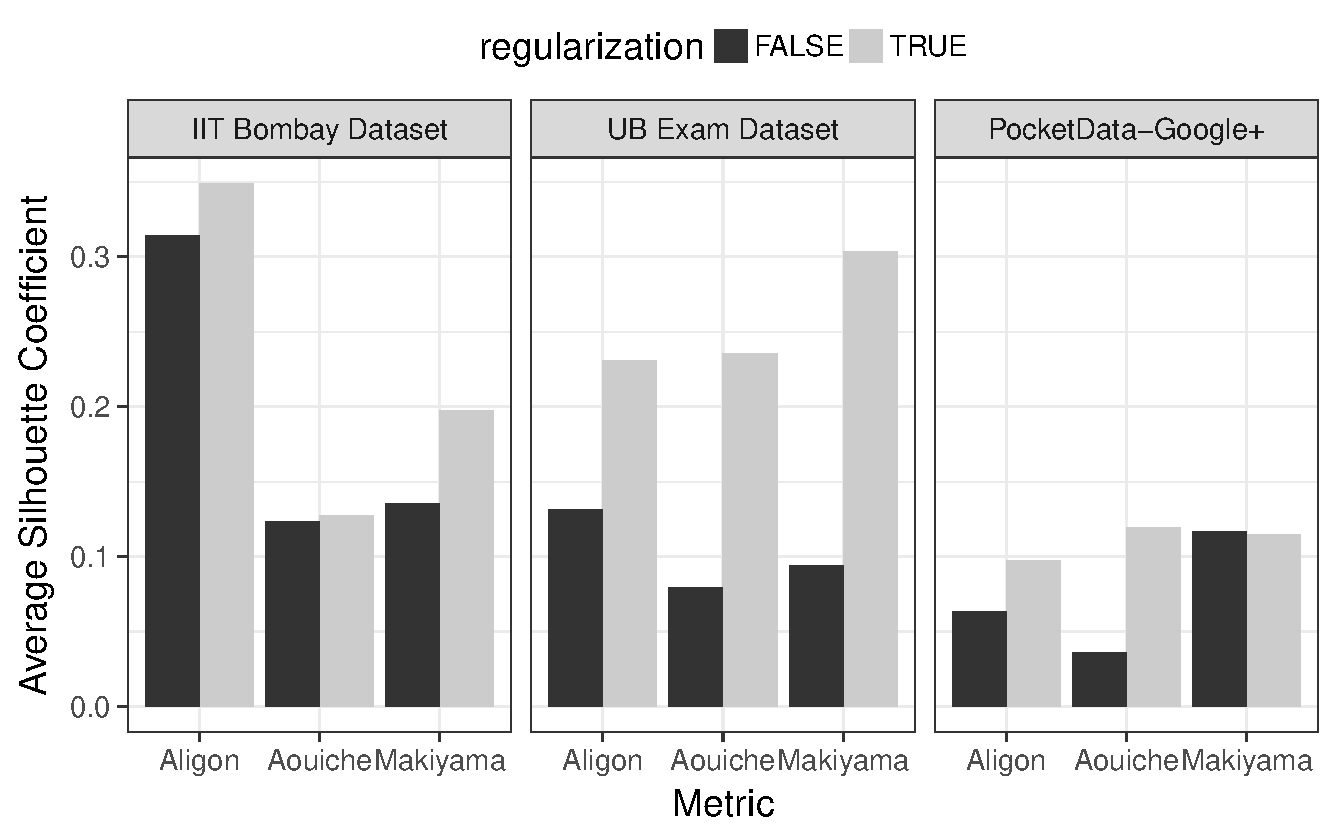
\includegraphics[width=\textwidth]{graphics/silhouette2}
        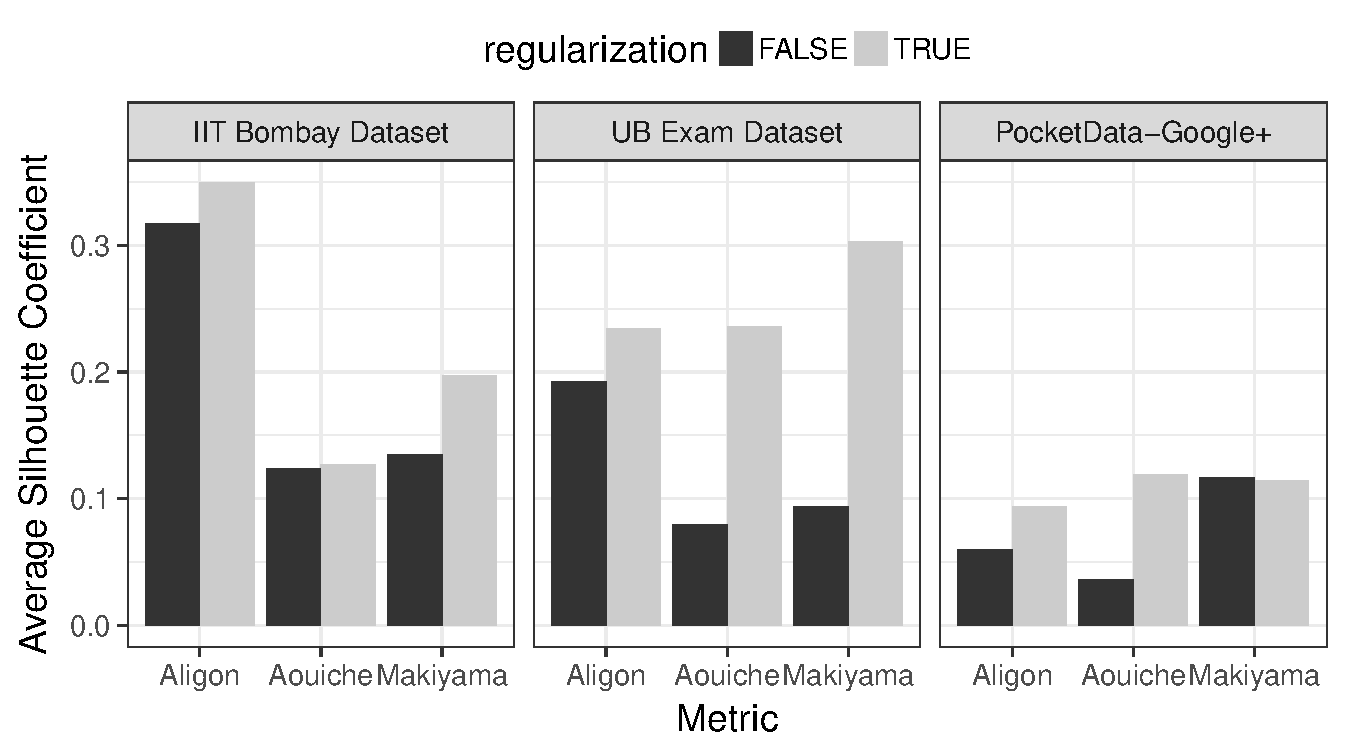
\includegraphics[width=\textwidth]{TKDE-QuerySimilarity/graphics/compare_silhouette}
        \caption{Average Silhouette Coefficient\\(\textit{larger} values are better)}
    \end{subfigure}%
    ~
    \begin{subfigure}[b]{0.48\textwidth}%{0.322\textwidth}
        \centering
        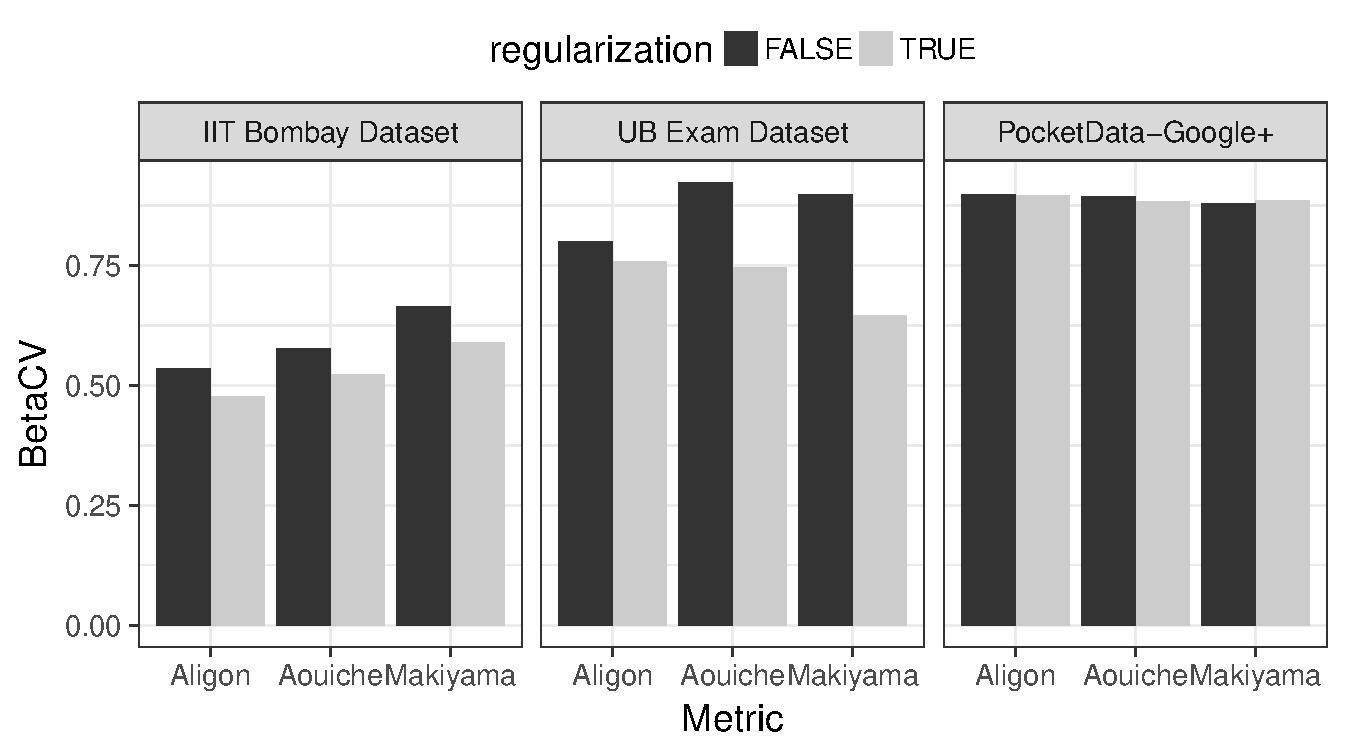
\includegraphics[width=\textwidth]{TKDE-QuerySimilarity/graphics/compare_betacv}
        \caption{BetaCV\\(\textit{smaller} values are better)}
    \end{subfigure}
    ~
    \begin{subfigure}[b]{0.48\textwidth}%{0.322\textwidth}
        \centering
        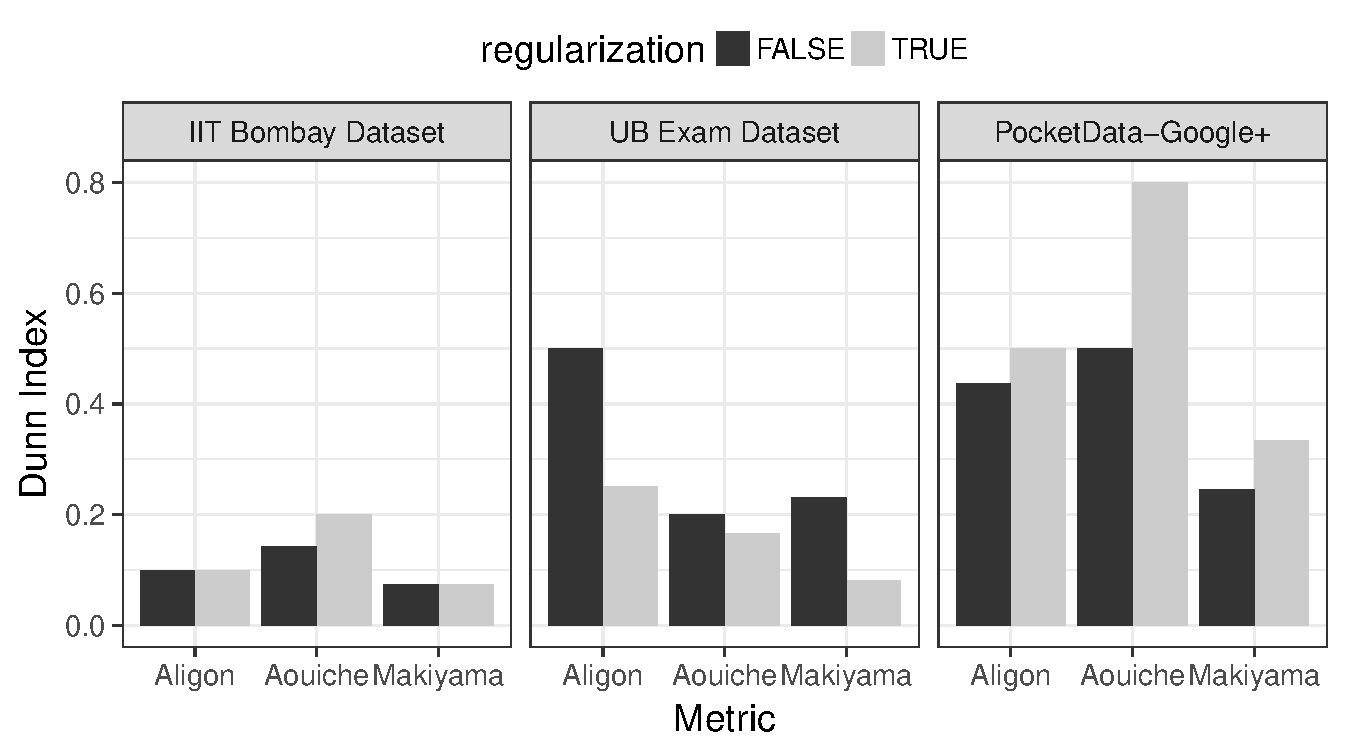
\includegraphics[width=\textwidth]{TKDE-QuerySimilarity/graphics/compare_dunn}
        \caption{Dunn Index\\(\textit{larger} values are better)}
    \end{subfigure}
    \caption{Clustering validation measures for each metric with and without regularization step}
    \label{fig:comparison2}
\end{figure*}

The black columns in Figure~\ref{fig:comparison2} show a comparison of three similarity metrics using each of the three quality measures (Average Silhouette Coefficient, BetaCV and Dunn Index).  
As can be seen in Figure~\ref{fig:comparison2}, Aligon seems to work the best for both IIT Bombay and UB Exam dataset while achieving second-best for PocketData-Google+ dataset under the Average Silhouette Coefficient measure. 
When considering BetaCV measure, Aligon also attains the best result for both IIT Bombay and UB Exam dataset while having comparable result for PocketData-Google+ dataset.
Aligon also performs well on the Dunn Index, coming in first on UB Exam dataset, and second-best for IIT Bombay and PocketData-Google+ dataset.
Especially given that the Dunn Index measures only worst-case performance, Aligon's metric seems to be ideal for our workloads.
This shows that even a fairly simple approach can capture task similarity well. 

\begin{figure*}[h!]
	\captionsetup[subfigure]{justification=centering}
    \centering
    \begin{subfigure}[b]{0.45\textwidth}%{0.32\textwidth}
        \centering
        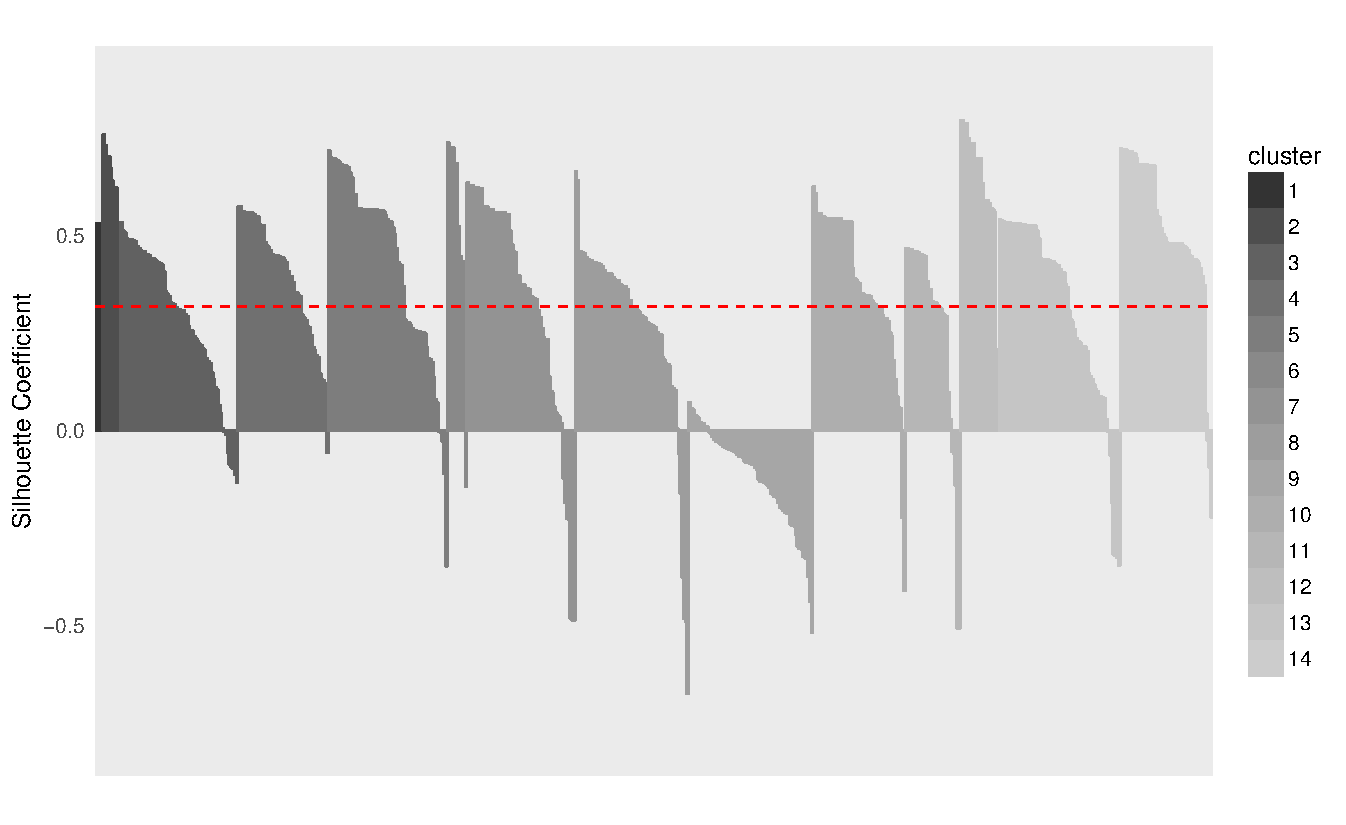
\includegraphics[width=\textwidth]{TKDE-QuerySimilarity/graphics/sil_bombay_Aligon}
		\caption{IIT Bombay dataset}
        \label{fig:sil_aligon:bombay}
    \end{subfigure}
    ~
    \begin{subfigure}[b]{0.45\textwidth}%{0.32\textwidth}
        \centering
        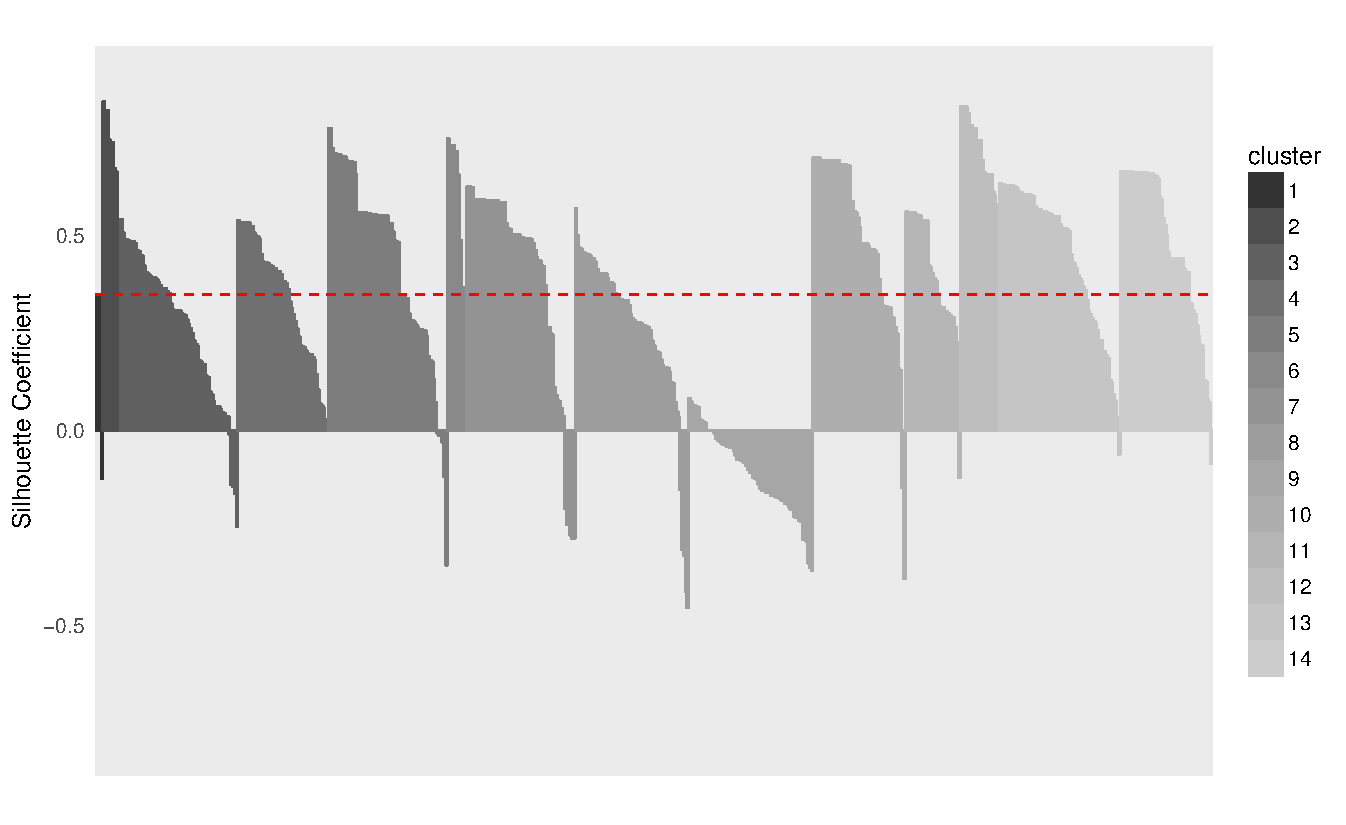
\includegraphics[width=\textwidth]{TKDE-QuerySimilarity/graphics/sil_bombay_Aligon_regularization}
		\caption{IIT Bombay dataset}
		\label{fig:sil_aligon:bombay_preprocess}
    \end{subfigure}
    \\
    \begin{subfigure}[b]{0.45\textwidth}%{0.32\textwidth}
        \centering
        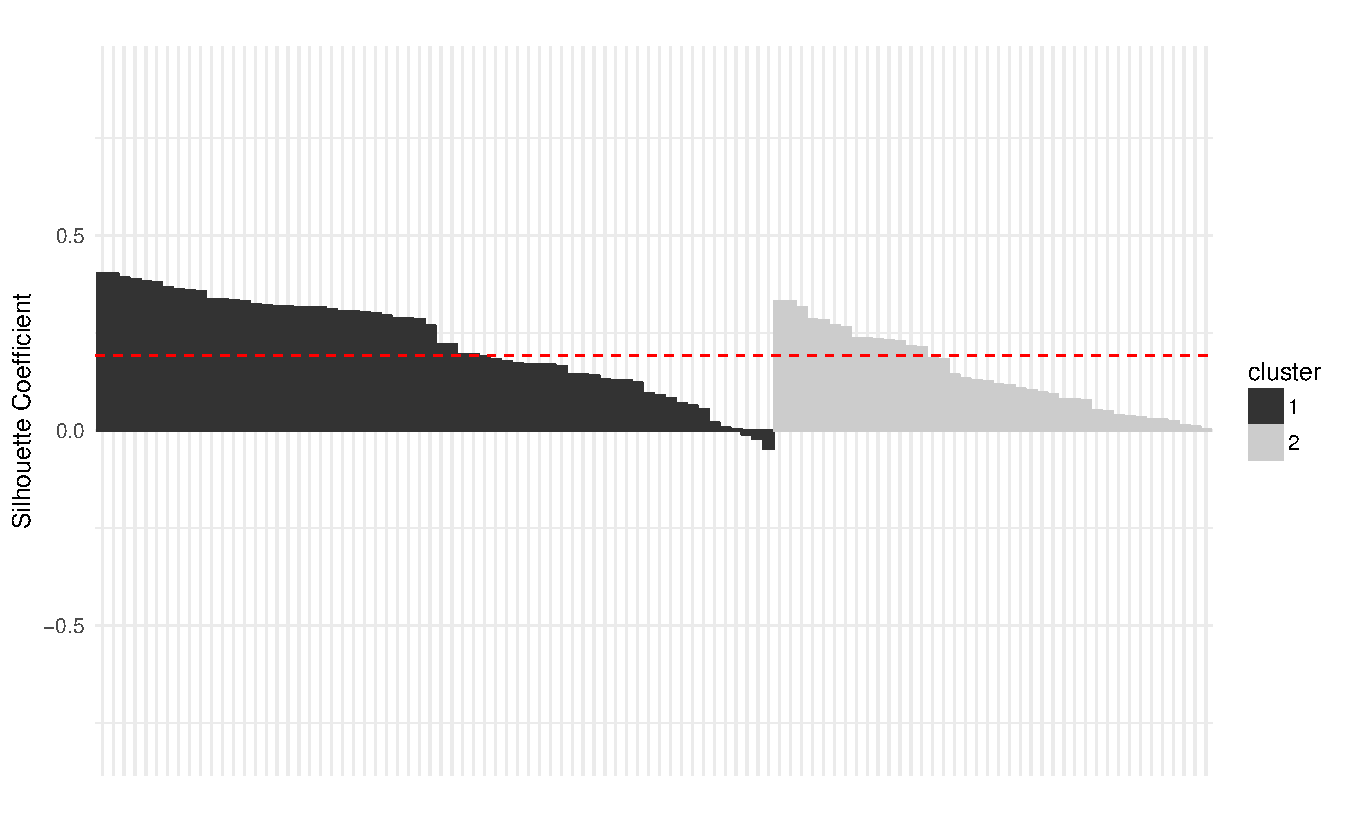
\includegraphics[width=\textwidth]{TKDE-QuerySimilarity/graphics/sil_ub_Aligon}
        \caption{UB Exam dataset}
        \label{fig:sil_aligon:local}
    \end{subfigure}
    ~
	\begin{subfigure}[b]{0.45\textwidth}%{0.32\textwidth}
        \centering
        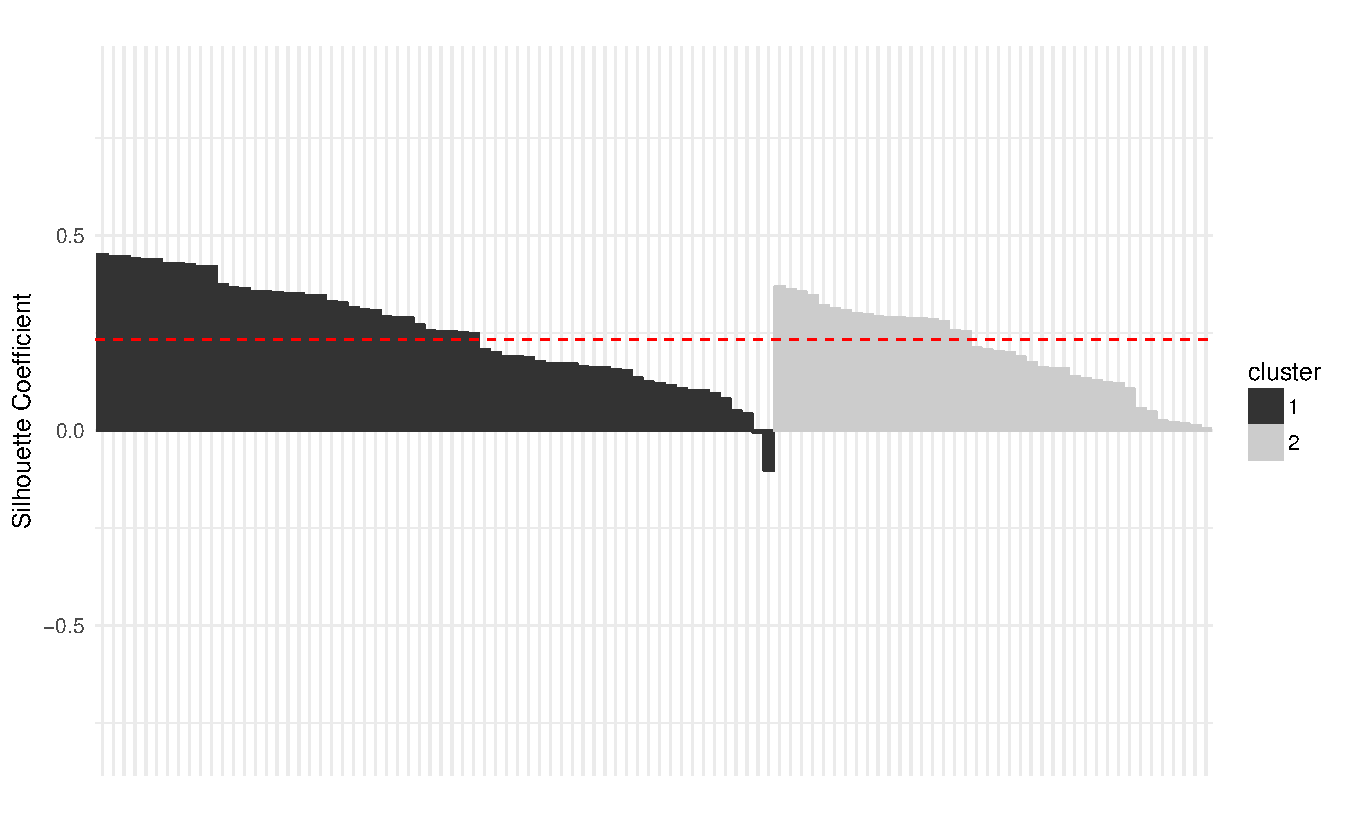
\includegraphics[width=\textwidth]{TKDE-QuerySimilarity/graphics/sil_ub_Aligon_regularization}
        \caption{UB Exam dataset}
        \label{fig:sil_aligon:local_preprocess}
    \end{subfigure}    
    \\
    \begin{subfigure}[b]{0.45\textwidth}%{0.32\textwidth}
        \centering
        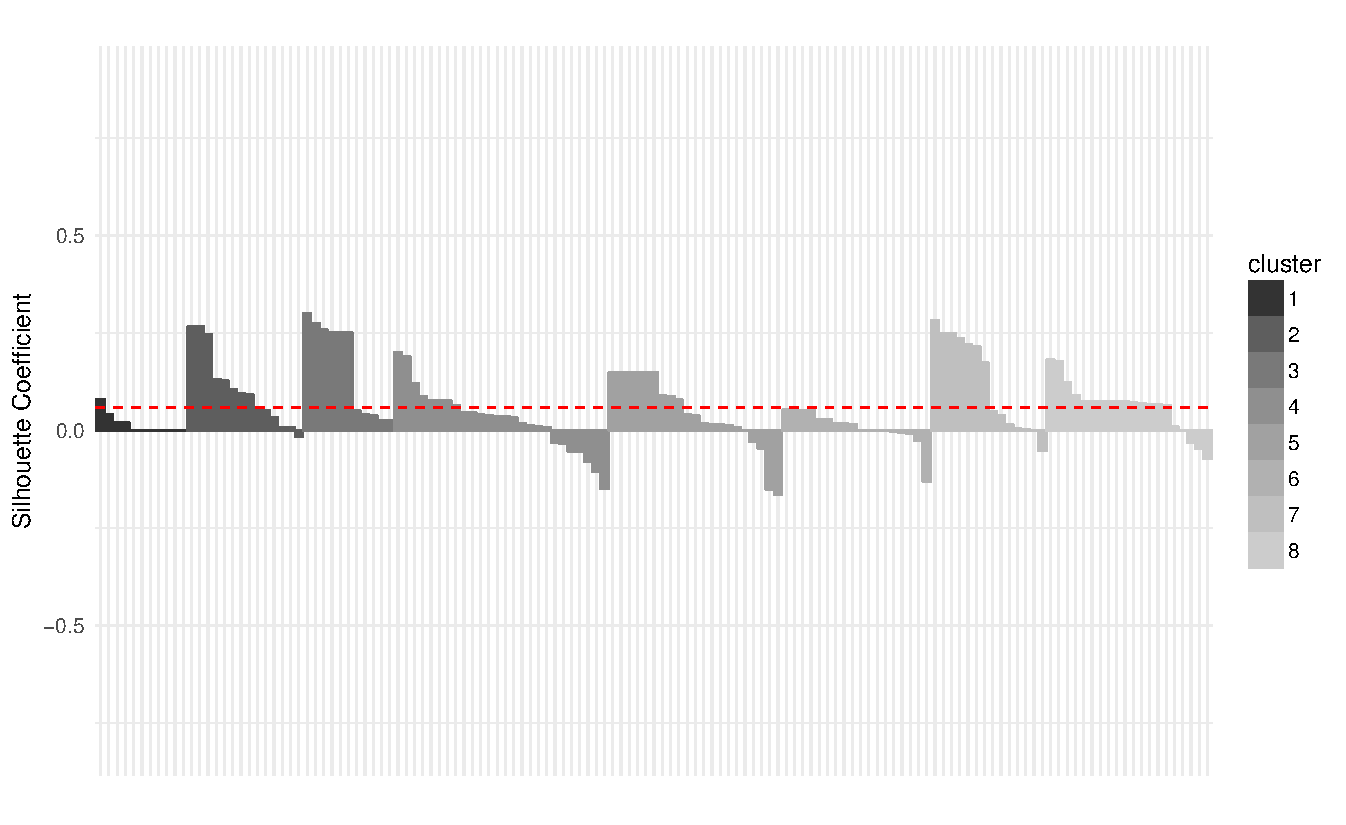
\includegraphics[width=\textwidth]{TKDE-QuerySimilarity/graphics/sil_googleplus_Aligon}
        \caption{PocketData-Google+ dataset}
        \label{fig:sil_aligon:googleplus}
    \end{subfigure}
    ~
    \begin{subfigure}[b]{0.45\textwidth}%{0.32\textwidth}
        \centering
        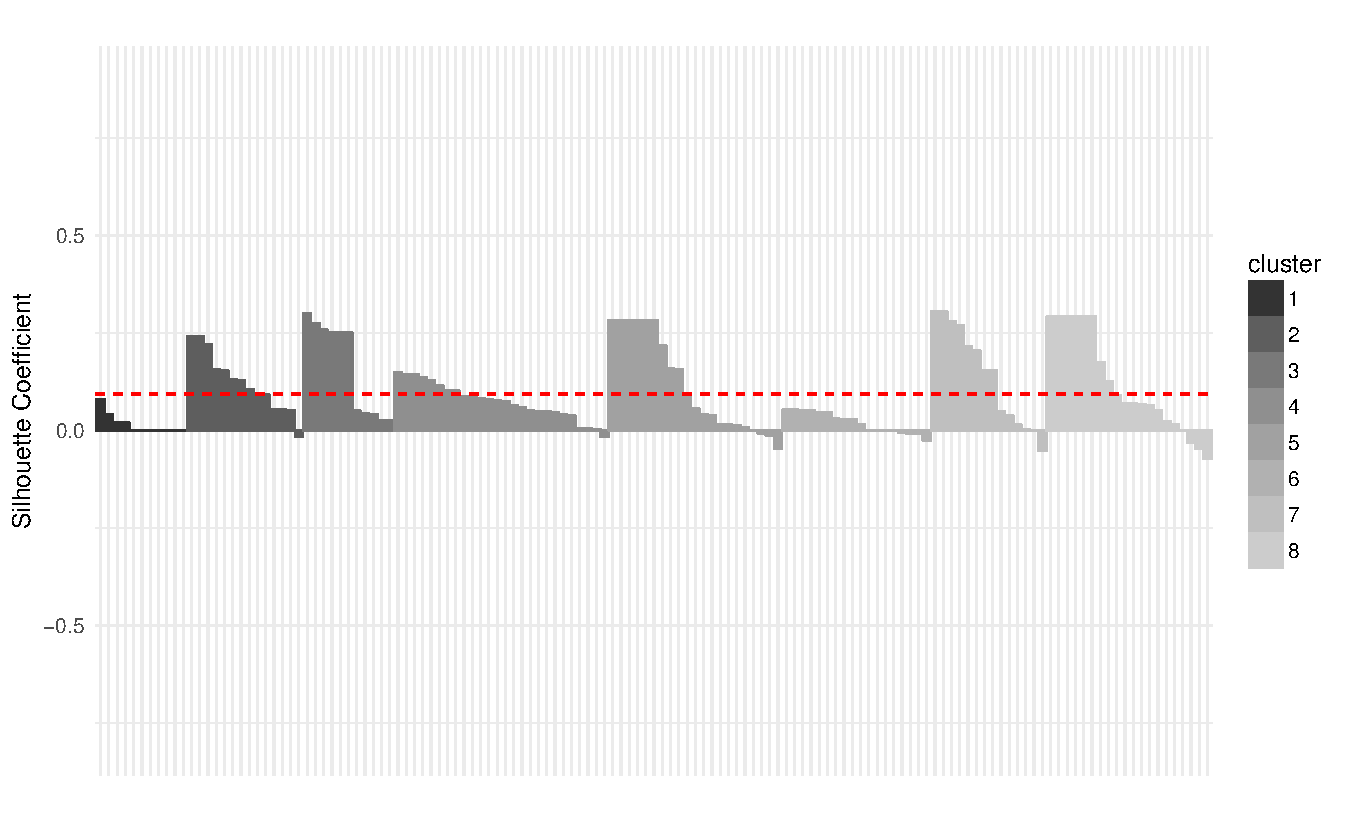
\includegraphics[width=\textwidth]{TKDE-QuerySimilarity/graphics/sil_googleplus_Aligon_regularization}
        \caption{PocketData-Google+ dataset}
        \label{fig:sil_aligon:googleplus_preprocess}
    \end{subfigure}
    \caption{Distribution of silhouette coefficients when using Aligon's similarity without regularization (a,c,e), and when regularization is applied (b,d,f)}
    \label{fig:sil_aligon}
    \label{fig:sil_aligon_preprocessed}
\end{figure*}

For a closer look of Aligon's similarity metric, Figure~\ref{fig:sil_aligon}(a,c,e) shows the distribution of Silhouette coefficients for each query and their respective tasks.   
Recall that the silhouette coefficient below 0 effectively indicates a query closer to another cluster than its own, or a query that would be mis-classified.  The further below zero, the greater the error.  
For the UB Exam dataset (Figure~\ref{fig:sil_aligon:local}), the majority of queries would have been successfully classified, and only a small fraction exhibit minor errors.
For the PocketData-Google+ dataset (Figure~\ref{fig:sil_aligon:googleplus}), there are some erroneous queries in cluster 4, 5 and 6 while cluster 1, 2, 3, 7 and 8 have very few errors.
For the Bombay dataset (Figure~\ref{fig:sil_aligon:bombay}), the distribution of errors varies.  
Cluster 1, 2, 4, 6, 12 and 14 exhibit virtually no error, while cluster 7, 8, and 9 exhibit particularly egregious errors.

\subsection{Evaluation of feature engineering}
\label{subsec:evaluation}
The effectiveness of regularization is evaluated by applying it to each of the three metrics described in Section~\ref{sec:background}.
The quality evaluation scheme is used to compare the quality of each measure both with and without feature engineering.

Figure~\ref{fig:comparison2} shows the values of three validation measures for each of the three similarity metrics, both with and without regularization.
As shown in Figure~\ref{fig:comparison2}, regularization significantly improves the Average Silhouette Coefficient and BetaCV measures for all similarity metrics except for the case of Makiyama similarity metric with PocketData-Google+ dataset.
The Dunn index is relatively unchanged or little improved for the IIT Bombay and PocketData-Google+ dataset and shows slight signs of worsening with regularization on the UB Exam dataset. To understand the reason of worse Dunn Index, Figure~\ref{fig:sil_aligon:local} (original) is compared with Figure~\ref{fig:sil_aligon:local_preprocess} (with regularization). 
The Silhouette Coefficient for answers that are originally positive in each question are considerably increased, and for answers that are originally negative (regarded erroneous) are even more decreased as a result of regularization, since it reduces the query structure diversity which leads to separating queries better.
In other words, for erroneous answers with negative Silhouette Coefficients, distance metrics like Aligon distinguish them further apart from answers with positive Silhouette Coefficients after regularization. 
Since erroneous answers are treated as the `worst cases' for each question, the Dunn Index which measures worst case performance naturally gets worse.

\subsubsection{Per-Query Similarity}
Figure~\ref{fig:sil_aligon_preprocessed}(b,d,f) shows the distributions of silhouette coefficients for the Aligon similarity metric after regularization is applied.  
For IIT Bombay dataset, comparing against Figure~\ref{fig:sil_aligon:bombay} there is a slight improvement at the tail end of clusters 9, 11, 12, 13 and 14 --- several of the negative coefficients have been removed.  
Furthermore, positive matches have been improved, particularly for cluster 7, 9, 10, 12 and 13.  
Finally, there has been a significant reduction in the degree of error in cluster 10.  
Cluster 10 is a particularly egregious case of aliasing, as the correct answer involves two self-joins in the same query.
As a result, aliasing is a fundamental part of the correct query answer, and our rewrites could not reliably create a uniform set of alias names.
In the UB Exam and PocketData-Google+ datasets, the improvement provided by regularization can be seen for queries with both positive and with negative values of $s(i)$.


\subsection{Case Study}
As part of the analysis, empirical explanations for query errors are provided by manual work, in particular for queries where $s(i) < 0$ for all three similarity metrics. 
Namely, queries that are too far apart from the clusters they belong are manually examined, and the reasons for mis-classification are categorized. 
We then investigate how the regularization process particularly affect these queries. 

Almost all of these egregiously mis-classified queries appear in the IIT Bombay dataset, the distribution of which is summarized in Table~\ref{tab:errorsources}.
The PocketData-Google+ dataset includes no egregiously mis-classified queries, while the UB Exam dataset includes only one such query (which tagged as a case of \textbf{Contextual equivalence}).
Each egregiously mis-classified query is tagged with an explanation that justifies why the query has a low s(i). 
Tags were drawn from the following list:

\smallskip
\tinysection{Ground-truth error} A student's response to the question may have been legitimately incorrect. This is a query that is correctly classified as an outlier.
For example: 
{\footnotesize
\begin{verbatim}
SELECT *
FROM (SELECT id, name, time_slot_id
 FROM (SELECT *
  FROM (SELECT *
   FROM student
    NATURAL JOIN takes) b1) a, section
   WHERE a.course_id = section.course_id) a1
\end{verbatim}
}
This query was attempting to complete the task \textit{``Find the ID and names of all students who have (in any year/semester) taken two courses in the same timeslot.''}

\smallskip
\tinysection{Nested subquery} A student's response is equivalent to a legitimately correct answer but uses nested subqueries such that a heuristic distance metric cannot recognize.
For example: 
{\footnotesize
\begin{verbatim}
SELECT id, name FROM student
WHERE id IN (SELECT DISTINCT s.id
 FROM (SELECT * FROM takes NATURAL JOIN section) s,
  (SELECT * FROM takes NATURAL JOIN section) t
 WHERE s.id = t.id
  AND s.time_slot_id = t.time_slot_id
  AND s.course_id <> t.course_id)
\end{verbatim}
}

Here, the subquery nesting structure is significantly different from other queries for of the same question.

\smallskip
\tinysection{Aliasing} Aliasing (e.g., \texttt{AS} in SQL) breaks a distance metric that relies on attribute and relation names.
For example:
{\footnotesize
\begin{verbatim}
SELECT DISTINCT student.id, student.name
FROM student, takes, section AS a, section AS b
WHERE student.id = takes.id
  AND takes.course_id = a.course_id
  AND takes.course_id = b.course_id
  AND a.course_id <> b.course_id
  AND a.time_slot_id = b.time_slot_id
\end{verbatim}
}

The student's use of \texttt{a} and \texttt{b} make this query hard to distinguish from other queries that may use other names for the attributes.

\smallskip
\tinysection{Insufficient features} Relevant query components are not sufficiently captured as features for a heuristic distance metric to distinguish between answers from sufficiently similar questions.

\smallskip
\tinysection{Too many features} Irrelevant query components create redundant features that artificially increase the distance between the query and cluster center.
For example:
{\footnotesize
\begin{verbatim}
SELECT DISTINCT student.name, takes.id, 
                s1.course_id, s2.course_id
FROM section AS s1, section AS s2, takes, student
WHERE takes.course_id = s1.course_id
  AND s1.course_id <> s2.course_id
  AND s1.time_slot_id = s2.time_slot_id
  AND s1.semester = s2.semester
  AND s1.year = s2.year
  AND takes.sec_id = s1.sec_id
  AND s1.semester = takes.semester
  AND s1.year = takes.year
  AND student.id = takes.id
  AND s2.time_slot_id = s2.time_slot_id
  AND takes.sec_id = s2.sec_id
  AND s2.semester = takes.semester
  AND s2.year = takes.year
\end{verbatim}
}

\smallskip
\tinysection{Contextual equivalence} Establishing query equivalence to properly clustered queries requires domain-specific knowledge not available to the distance metric (e.g. attribute uniqueness).
For example:
{\footnotesize
\begin{verbatim}
SELECT student.id, student.name
FROM student
WHERE student.id
  IN (SELECT takes.id
    FROM takes, section
    WHERE takes.course_id = section.course_id
      AND takes.sec_id = section.sec_id
      AND takes.semester = section.semester
      AND takes.year = section.year
    GROUP BY takes.id,
        takes.semester,
        takes.year,
        section.time_slot_id
    HAVING count(*) > 1)
\end{verbatim}
}

\begin{table}[h!]
%\vspace{-3mm}
\centering
\begin{tabular}{ccccccc}
\toprule
 \textbf{\begin{tabular}[c]{@{}c@{}}Cause\end{tabular}} & \textbf{\begin{tabular}[c]{@{}c@{}}Erroneous \\queries \\ Without \\ Regularization\end{tabular}} & 
 \textbf{\begin{tabular}[c]{@{}c@{}}Erroneous \\queries \\ With \\ Regularization\end{tabular}}\\
 \midrule
 All queries & 33 (100\%) & 27 (100\%)\\% & 1 (100\%) & 1 (100\%) & 0 (100\%)& 0 (100\%)\\  
 Ground-truth quality & 14 (42.4\%) & 14 (51.8\%)\\% & 0 (0\%) & 0 (0\%) & 0 (0\%) & 0 (0\%)\\ 
 Nested subquery & 7 (21.2\%) & 5 (18.5\%)\\% & 0 (0\%) & 0 (0\%) & 0 (0\%) & 0 (0\%)\\ 
 Aliasing & 8 (24.2\%) & 5 (18.5\%) \\%& 0 (0\%) & 0 (0\%) & 0 (0\%) & 0 (0\%)\\ 
 Insufficient features & 2 (6.0\%) & 1 (3.7\%)\\% & 0 (0\%) & 0 (0\%) & 0 (0\%) & 0 (0\%)\\ 
 Too many features & 1 (3.0\%) & 1 (3.7\%) \\%& 0 (0\%) & 0 (0\%) & 0 (0\%) & 0 (0\%)\\ 
 Contextual equivalence & 1 (3.0\%) & 1 (3.7\%)\\% & 1 (100\%) & 1 (100\%) & 0 (0\%) & 0 (0\%)\\
 \bottomrule
\end{tabular}
\vspace{-2mm}
\caption{Empirical error reasons for IITBombay Dataset}
\label{tab:errorsources}
%\vspace{-3mm}
\end{table}

Table~\ref{tab:errorsources} shows the primary reasons why these queries could not be classified correctly. 
Note that there may be more than one reason for a query to be placed in a different cluster, but in Table~\ref{tab:errorsources}, only the empirically determined primary reason is given.

Many of the queries with low silhouette coefficients are identified as incorrect answers for the task given. 
These answers directly affect the ground-truth quality, therefore reduce the average silhouette coefficient. 
Another reason for erroneous queries with low silhouette coefficients is because of aliasing. 
Although it is convenient for user to use aliases in the query to refer to a particular item, it is difficult for a machine to approximate the tasks the query authors are trying to accomplish since different query authors have different ways to name particular items in the query. 
This problem is particularly prevalent in question 9 of the IIT Bombay dataset.

Although the distribution of the error reasons are expected to change, all the tags provided in this section can generically be applied to other query logs given a ground-truth. 
The regularization method cannot be expected to fix errors originating from mis-classifications in ground-truth since they do not actually share any similarities with the cluster. 

After the regularization process, the silhouette coefficient under all three similarity metrics for each query is computed again and the result yields an 18\% overall reduction in number of erroneous queries ($s(i) < 0$)  in the IIT Bombay dataset. 

\subsection{Analysis of regularization by module}
\label{subsec:modules}
In subsection~\ref{subsec:evaluation}, the overall effect of regularization on query similarity is analyzed.  
However, as described in Section~\ref{sec:system}, regularization is composed of many different transformation rules.  
In this experiment, these rules are grouped into four separate modules before their impact on the clustering quality is inspected. 
One may observe that Commutative Operator Ordering is guaranteed to provide benefit in structure similarity comparison, hence it is included in all four modules. 
In addition, there are dependencies between rules that require them to operate one before another. 
For example, one should better apply Syntax Desugaring and then DNF Normalization to simplify the boolean expression in WHERE clause before OR-Union Transformation.
As another example, Exists Standardization should better be applied on nested sub-queries before we de-correlate them using Nested Query De-correlation.
As a result, the rules are grouped from Section~\ref{sec:system} into four modules:
\begin{enumerate}
\item \textit{Naming}: \textbf{Canonicalize Names and Aliases}
\item \textit{Expression Standardization}: \textbf{Syntax Desugaring}, \\\textbf{Exists~Standardization}, \textbf{DNF~Normalization}, \\\textbf{Nested~Query~Decorrelation}, \textbf{OR-Union~Transform}
\item \textit{FROM-Nesting}: \textbf{Flatten FROM-Nesting}
\item \textit{Union Pullout}: \textbf{OR-UNION Pullout}
\end{enumerate}
\textbf{Commutative Operator Ordering} is included in all modules.

Figure~\ref{fig:module} provides a comparison of each module in regularization. 
From this figure, one can observe that, since students use different names/aliases for their convenience when constructing queries, the \textit{Naming} module is the most effective one in terms of improving clustering quality for IIT Bombay and UB Exam datasets. 
On the other hand, for PocketData-Google+ dataset, names are already canonicalized as they are machine-generated. 
In this case, \textit{Expression Standardization} seems to be the most effective module, especially when using Aligon or Aouiche as similarity metric. 
In PocketData-Google+ dataset, referred tables and boolean expressions in the queries are both informative in distinguishing between different query categories or clusters. For this reason, Makiyama similarity metric which considers both works well even without regularization while Aligon and Aouiche can get commensurate performance only after applying \textit{Expression Standardization} module. 

Note that in Figure~\ref{fig:module}, \textit{Expression Standardization} makes Average Silhouette Coefficient worse in some cases for IIT Bombay and UB Exam data sets. 
The performance degradation is majorly due to \textit{feature duplication}. 
More specifically, consider the example query with \textit{Expression Standardization}.
\begin{example}
Syntax Desugaring with OR-UNION transform
{\footnotesize
\begin{enumerate}
\item\begin{verbatim}
SELECT name FROM usr WHERE 
rank IN {'admin','normal'}
\end{verbatim}
\item\begin{verbatim}
SELECT name FROM usr WHERE 
rank = 'admin' OR rank = 'normal'
\end{verbatim}
\item\begin{verbatim}
SELECT name FROM usr
WHERE rank = 'admin'
UNION
SELECT name FROM usr
WHERE rank = 'normal' 
\end{verbatim}
\end{enumerate}
}
\end{example}
Query (1) is transformed into (2) by syntax~desugaring and then into (3) by OR-UNION~Transform. From (1) to (2), feature \texttt{WHERE rank} has been replicated; From (2) to (3), features \texttt{SELECT name} and \texttt{FROM usr} have been duplicated. For expressions of the form: \texttt{X IN} $\{x_1,x_2,\dots,x_n\}$, feature duplication becomes dominant when $n$ grows large. 
In Figure~\ref{fig:module}, Aligon and Makiyama suffer from feature duplication brought by~\textit{Expression Standardization} in some cases while Aouiche does not. 
Because Aouiche records feature existence instead of occurrence in its vector. 
Although in some cases such as this, simply replacing feature occurence with existence solves the problem of feature duplication, feature occurence can also be a good indicator for the interests of the query. 
It is believed that this problem can be addressed with exploration of feature weighting strategies. 
Therefore, the problem of feature duplication will be further explored as a part of feature weighting strategies in our future work.

\begin{figure*}[h!]
    \vspace*{-2mm}
    \centering
    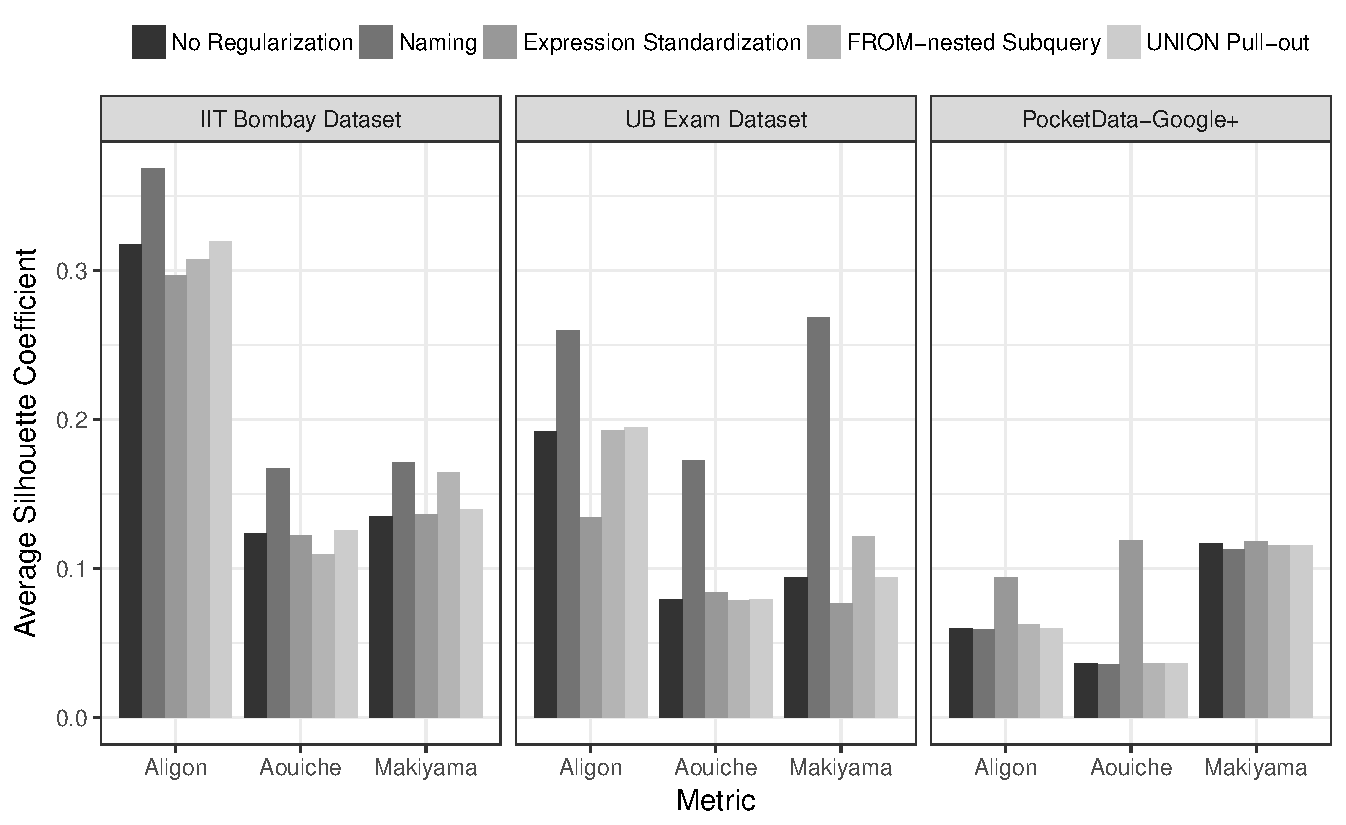
\includegraphics[width=0.70\textwidth]{TKDE-QuerySimilarity/graphics/module}%[width=\columnwidth]{graphics/module}
	\caption{Effect of each module in regularization}
    \label{fig:module}
    %\vspace*{-4mm}
\end{figure*}

